\documentclass[11pt]{article}
\usepackage{mathtools}
\usepackage{mdframed}
\usepackage{fullpage}
\usepackage{amsfonts}
\usepackage{tikz}            % if you delete this, you will have trouble with the included picture. You can delete the picture.




\newcommand\name{John Vincent} %%%%%%%%%%%%%%  WRITE YOUR NAME HERE



\newcounter{excounter}
\setcounter{excounter}{1}
\newcommand\question[2]{\vskip 1em  \noindent\textbf{\arabic{excounter}\addtocounter{excounter}{1}:} \emph{#1} \noindent#2}


% You can also erase this if you do not have package hancyhdr
% Fancy footnote.........
\usepackage{fancyhdr}  %% If it does not work with your latex installation, you may just delete this...
\pagestyle{fancy}
\usepackage{lastpage}
\rfoot{\name, page \thepage/\pageref{LastPage}}
\cfoot{}
\rhead{}
\lhead{}
\renewcommand{\headrulewidth}{0pt}
\renewcommand{\footrulewidth}{0pt}
\DeclarePairedDelimiter\ceil{\lceil}{\rceil}
\DeclarePairedDelimiter\floor{\lfloor}{\rfloor}



\begin{document}


  {\bf COMS 331  \hspace{1cm} HW 0\hfill \name}
  \vskip 2em


  \question{}

  \begin{mdframed}
    This is an inline equation: $x + y = 3$.\\
    This is a displayed equation: \begin{equation*}x + \frac{y}{z-\sqrt{3}}=2.\end{equation*}
    This is how you can define a piece-wise linear function:
      \[
        f(x) =
        \begin{cases}
          3x + 2 & \text{if $x < 0$}\\
          7x + 2 & \text{if $x \geq 0$ and $x < 10$}\\
          5x + 22 & \text{otherwise.}
        \end{cases}
      \]
    This is a matrix:
      \bgroup
        \def\arraystretch{1.5}%
        \begin{center}
          \begin{tabular}{|c|c|c|c|}
            \hline
            9 & 9 & 9 & 9 \\ \hline
            6 & 6 & 6 &   \\ \hline
            3 &   & 3 & 3 \\
            \hline
          \end{tabular}
        \end{center}
      \egroup
    \noindent This is a figure incorporated in a LaTeX file
    \begin{center}
      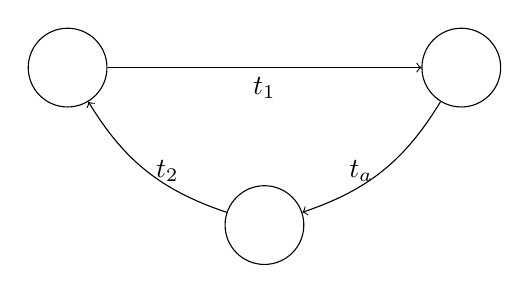
\begin{tikzpicture}
        \node[shape=circle,draw=black,minimum size=1cm] (A) at (0,2) {};
        \node[shape=circle,draw=black,minimum size=1cm] (B) at (5,2) {};
        \node[shape=circle,draw=black,minimum size=1cm] (C) at (2.5,0) {};

        \path [->] (A) edge node[below] {$t_{1}$} (B);
        \path [->] (B) edge[bend left=20] node[left] {$t_{a}$} (C);
        \path [->] (C) edge[bend left=20] node[right] {$t_{2}$} (A);
      \end{tikzpicture}
    \end{center}
  \end{mdframed}

  \question{}
    consider the function $ f(x) = \begin{cases}
                                    x/2 & \text{if $x$ is even}\\
                                    -\frac{x+1}{2} & \text{if $x$ is odd}\\
                                    0 & \text{if $x=0$}
                                 \end{cases}
                       $
    where $x\in \mathbb{N}$ and $f(x)\in \mathbb{Z}$. This function is a bijection between $\mathbb{N}$ and $\mathbb{Z}$, and
    since there is a bijection between them they must be equinumerious.

  \question{}
    assume that if a set $S$ is infinte that there can not exist a function $f$
    such that $f: S\to S$ and $f$ is surjective but not injective, or injective
    but not surjective. consider the function $g(x)=x^2$ over the the infinite
    set $f: \mathbb{N}\to\mathbb{N}$. the element $3$ in the set $\mathbb{N}$
    is a counter example to $g(x)$ being onto since $\sqrt{3}$ is not in $\mathbb{N}$.
    assume that there is some $x \ne y$ where $g(x) = g(y)$, that would mean
    that $x^2 = y^2$, but there are not values in $\mathbb{N}$ for which this is
    true since they are all positive proving that $g$ is one-to-one by contradicton.
    This makes $g$ an example of a function from and infinite set to itself
    that is one-to-one yet not onto. Now consider the function $h=x+2\floor{x/2}$ for
    $h: \mathbb{R}\to\mathbb{R}$ this function is not one-to-one and
    $x=1$ and $x=2$ are a counter example. It is onto though because every value
    in the range has two values in the domain that equal it. This makes $h$
    and example of a function that is onto, but not one-to-to. proving that
    an infinite set $S$ can have a fuction $f: S\to S$ that is injective but not
    surjective, and surjective but not injective by contradiction.

  \question{}
    $R$ is reflexive since if $m = n$ then $m-n = 0$ and $0 mod 3$ will always be $0$.\\
    $R$ can be shown to be symetric by direct proof.\\
    assume that for some random values $m,n\in\mathbb{N}$ where $(m-n) mod 3 = 0$ then $(n-m) mod 3$ must also equal $0$ since
    $n-m = -(m-n)$ so $(n,m)\in R$ if $(m,n)\in R$\\
    $R$ can be shown to be transitive by direct proof\\
    assume that from some rand values $a,b,c\in\mathbb{N}$ $(a,b)\in R$ and $(b,c)\in R$. this mean that $a-b = 3n$ and
    $b-c = 3m$ where $m$ and $n$ are unknown constants. this means that $a-c = 3n + 3m = 3(n+m)$. which means that
    $(a-c) mod 3 = 0$ and $(a,c)\in R$.\\
    since $R$ is relexive symetic and transitive it is an Equivalence relation, and its Equivalence classes are
    $\{0, 3, 6, 9, ...3n\}, \{1, 4, 7, ...3n+1\}, \{2, 5, 8, ...3n+2\}$ where $n\in\mathbb{N}$
  \question{}
    Proof by induction on $n$.\\
    \textit{Basis:} when n = 1 $\sum^{1}_{i=1} i^{2} = 1$ and $(2(1)+1)(1+1)(1)/6 = 1$  \\
    \textit{Induction hypothesis:} Assume that this holds true for all $n$ up to some value $m$\\
    \textit{Inductive step:}
    \begin{align}
      \sum^{n+1}_{i=1} i^{2} &= \frac{(2(n+1) + 1)(n+1+1)(n+1)}{6}\\
      (n + 1)^2+ \sum^{n}_{i=1} i^{2} &= \frac{(2n + 3)(n+2)(n+1)}{6}\\
      (6n^2 + 12n + 6) + (2n+1)(n+1)n &= (2n + 3)(n+2)(n+1)\\
      2n^3 + 9n^2 + 13n + 6 &= 2n^3 + 9n^2 + 13n + 6
    \end{align}
    which shows the property holds for $n+1$ proving $\sum^{n}_{i=1} i^2 = \frac{(2n + 1)(n+1)n}{6}$ by induction

\end{document}
